\documentclass[12pt,reqno]{amsart}
\usepackage[margin=1in]{geometry}                % See geometry.pdf to learn the layout options. There are lots.
\geometry{letterpaper}                   % ... or a4paper or a5paper or ... 
%\geometry{landscape}                % Activate for for rotated page geometry
%\usepackage[parfill]{parskip}    % Activate to begin paragraphs with an empty line rather than an indent
\usepackage{graphicx}
\usepackage[dvipsnames]{xcolor}
\usepackage{amssymb}
\usepackage{hyperref}
\usepackage{epstopdf}
%\usepackage{natbib}
\usepackage{color}
\usepackage{subcaption}
\usepackage{tikz}
\usepackage{url}
\usepackage[shortlabels]{enumitem}
\usepackage{amsmath}
\usetikzlibrary{graphs,graphs.standard}
\usepackage{verbatim}
\usepackage{subfigure}
\usepackage{float}
\usepackage{tabularx}
\usepackage{comment}


\DeclareGraphicsRule{.tif}{png}{.png}{`convert #1 `dirname #1`/`basename #1 .tif`.png}

%tikz specifications
\tikzstyle{vertex}=[circle, draw, inner sep=0pt, minimum size=6pt, fill=black]
\newcommand{\vertex}{\node[vertex]}

% Theorem Formatting Commands.
\theoremstyle{plain}
\newtheorem{thm}{Theorem}%[section]
%\newtheorem{lemma}{Lemma}[section]
\newtheorem{lemma}[thm]{Lemma}
\newtheorem{prop}[thm]{Proposition}
\newtheorem{cor}[thm]{Corollary}
\newtheorem{conj}[thm]{Conjecture}
\newtheorem*{thm*}{Theorem}
\newtheorem*{lemma*}{Lemma}
\newtheorem*{prop*}{Lemma}
\newtheorem*{cor*}{Corollary}
\newtheorem*{conj*}{Conjecture}

\theoremstyle{definition}
\newtheorem{defn}[thm]{Definition}
\newtheorem*{defn*}{Definition}
\newtheorem{ex}[thm]{Example}
\newtheorem{pr}[thm]{Problem}
\newtheorem{alg}[thm]{Algorithm}
\newtheorem{ques}[thm]{Question}

\theoremstyle{remark}
\newtheorem{rmk}[thm]{Remark}
\newtheorem*{obs}{Observation}

\title{Project Pickup}
\author{Mackenzie Bookamer \and Thalia Koutsougeras\\Tulane University}

\begin{document}

\maketitle

\section{Abstract}
In this project, we aim to utilize pre-trained language models (PLMs) to create a pickup line generator, which we call \textit{Pickup Master 9000}. By fine tuning the PLM GPT-2 from OpenAI with a wide variety of math and computer science pickup lines, we were able to generate coherent and subject relevant pickup lines. These generated pickup lines from our fine tuned model were both more coherent and subject relevant than those generated from the original PLM GPT-2 model. To facilitate user interaction with our model, we created a flask app that takes in user input and generates 2 pickup lines from our fine tuned model. 

\section{Introduction}
In today’s world, younger generations, especially STEM majors, seem to struggle with communicating in person in the dating world, tending to rely on mobile apps instead such as Tinder. A CS/math-themed pickup line generator can help ease this experience, by helping generate a pickup line in a pinch or helping you to practice your skills. This project aims to be very user friendly and incorporate user interaction to create an engaging experience. 

\section{Background/Related Work}
As part of a literature review, we examine relevant work being done on PLMs.

In Yeh, T. et al.'s \textit{Generating Original Jokes}\cite{yeh2018generating}, the authors examine how PLMs can gernerate jokes. This article was written before OpenAI and ChatGPT’s rise in popularity, so a PLM as robust as GPT-2 was not used. This paper also broadly focuses on all jokes, not topic-specific. This is where our project differs and makes it unique. It does give good ideas about how to validate and evaluate our output by having users compare the output to a common, human-generated output and determine which they like better. 


In Li, J. et al.'s \textit{Pretrained Language Models for Text Generation: A Survey}\cite{li2022pretrained}, the authors explain in detail PLM’s, starting broadly and then delving into the steps involved. The authors explain how to encode an input, describe different methods of fine-tuning, and challenges implicated in the process.


In Akbar, N. et al.'s \textit{Deep Learning of a Pre-trained Language Model’s Joke Classifier Using GPT-2}\cite{akbar2021deep}, the authors analyze joke classification. This article focuses on comparing the accuracy of classification models – namely BERT, CNN, and RNN – to correctly identify a joke generated from a PLM – GPT-2. They utilize fine-tuning algorithms on GPT-2 to generate the jokes, which is what we aim to do. 


In Radford, A. et al.'s \textit{Improving Language Understanding by Generative Pre-Training}\cite{radford2018improving}, the authors talk about fine tuning a PLM. The main point of this article is using generative pre-training of a language model, followed by discriminative fine-tuning. This could be useful to us because we could possibly pre-train our PLM with English jokes and specific category definitions, and then fine-tune with the category-specific pickup lines.


In Hempelmann, C. et al.'s \textit{Computer, Tell Me a Joke ... but Please Make it Funny: Computational Humor with Ontological Semantics}\cite{hempelmann2006computer}, the authors analyze generated jokes semantically. This article is different from the rest as it focuses primarily on the linguistic side of jokes and humor – the underlying theory behind the models proposed above. When evaluating the pick-up lines generated by our project, we can use the semantics presented in this article to objectively classify jokes.

\section{Data}
All of our data comes from 12 different websites such as Reddit and various blog posting sites, including 613 CS pickup lines and jokes from 5 different websites and 280 math pickup lines from 7 different websites. Together, we gathered 893 lines of data stored in 1 CSV-UTF8 file with no labels (the Data Collator handles the labels). 


\section{Approach}
Ultimately, our final product consists of a Flask app where the user can type in a fragment of a sentence and receive back a completed sentence, or can type in a question and receive an answer. 

Our project focuses on fine-tuning a pretrained GPT-2 model pulled from the Hugging Face model hub to the data we described above. We chose GPT-2 (medium) because it is still a robust dataset to work with efficiently – about 350 million parameters. We originally spent a good bit of time experimenting with the GPT-2 model by downloading it from the OpenAI repo and investigating how different parameters like temperature and top\_p affected the generated text outcome.

Through the HuggingFace transformers library, we also accessed the function GPT2Tokenizer. After loading in our pre-trained model and tokenizer in our $finetune.py$ file, we split the data into a train-test split with an 80-20 respective divide. The tokenizer was configured to use the end-of-sequence token as the padding token, as we noticed many generation tasks use to keep input sequences in a batch to the same length. We then pass this data through the tokenizer, which splits the input into individual tokens and maps each token to its unique UTF-8 ID that the GPT-2 model can then process. This process of tokenization is vitally important because it allows us to specifically train our GPT-2 model to generate text that is similar to our text of interest: STEM pickup lines and jokes. 

We then convert our data into a Dataset, which we found out is more efficient in data loading and processing, and has a standardized format compatible with Hugging Face's transformers library. The features of this Dataset object are the id's and the attention masks from the tokenizer, where the attention masks tell the model to ignore the pad tokens.

In order to finally fine-tune our model, we implement the Trainer class from the HuggingFace transformers library which abstracts the process of computing loss functions, making it more user friendly. As the model trains with each epoch, a new cross-entropy loss is calculated utilizing our train and test data sets. We also threw in some hyperparameters into the training arguments that we experimented with, such as the learning rate, weight decay, and number of epochs. Interestingly enough, we ran 10 epochs and saw that the loss was the lowest at the third epoch. Another important feature implemented with the Trainer class is the Data Collator, which handles our batch processing and padding. For one batch, the collator splits up the tokens such that the label sequence is shifted by one token compared to the input sequence. 

At this point, we are finally ready to train our data with $trainer.train()$! We also make sure to save the results of this model so that we can use it for generation.

\begin{figure}[H]
\centering
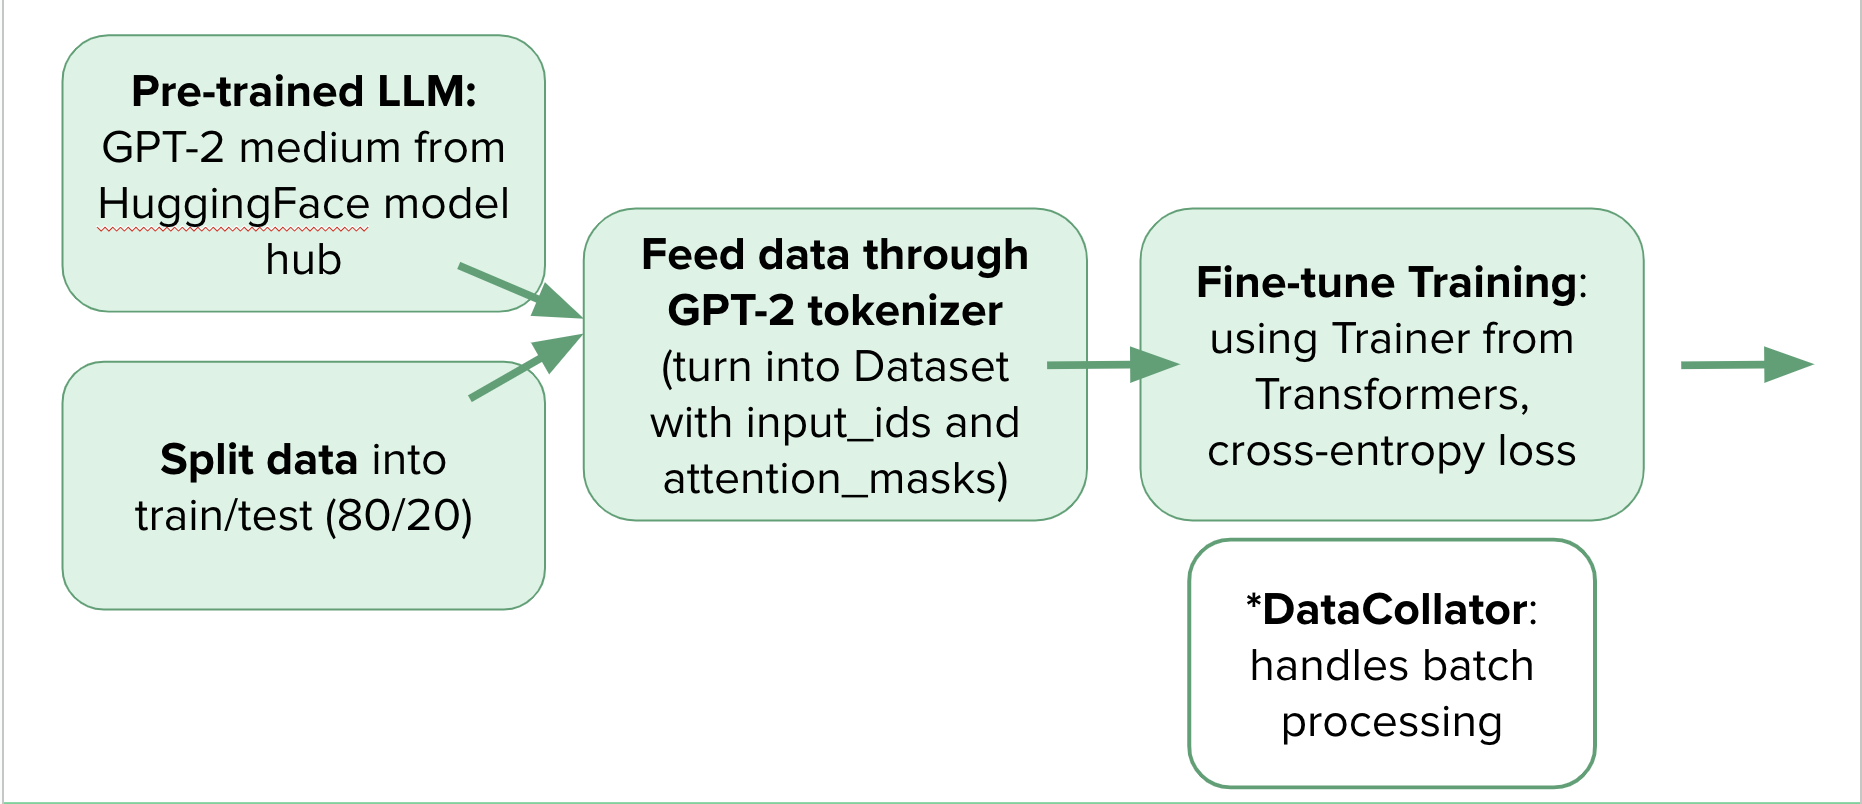
\includegraphics[width=0.75\textwidth]{pictures/fine tuning.png}
\caption{Summary of our fine tuning methods.}
\end{figure}

In order to generate our new pickup line, we load in our saved model and the same tokenizer in our $generation.py$ file. We then tokenize the user's input to convert it into the token\_ids format so that it can be fed back through the model. When we call $model.generate()$, we also feed it some other parameters that we've played around with such as temperature (randomness variable) and max\_length. One feature to highlight here is the use of top\_k sampling, which generates the top k most likely tokens at each step. We had previously tried out beam search as our decoding strategy, which we found produced too repetitive generated samples. We also generated 5 samples with each prompt. We also adapted this code to work with our Flask app as described in the Experiment section.

\begin{figure}[H]
\centering
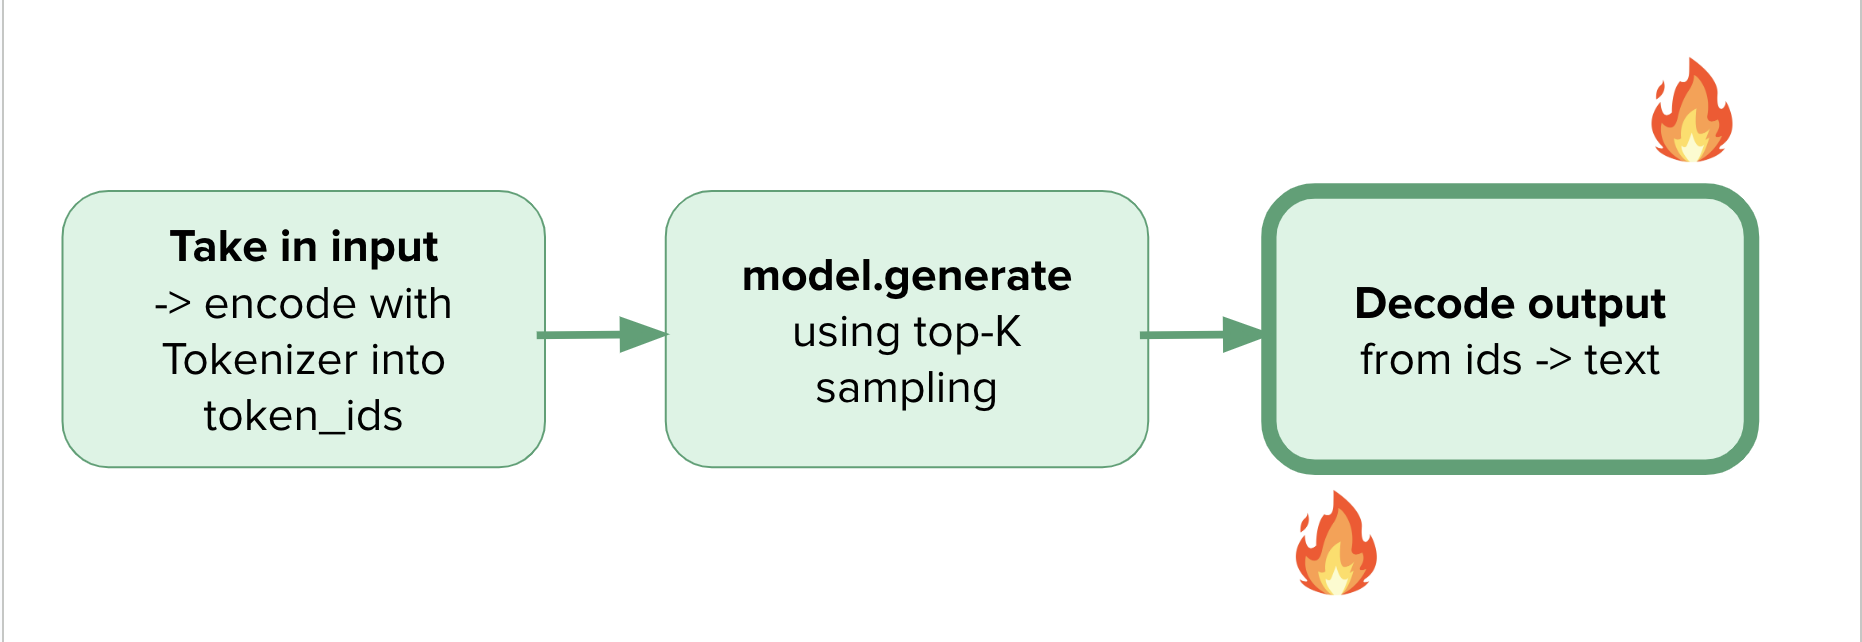
\includegraphics[width=0.75\textwidth]{pictures/generate.png}
\caption{Summary of our generation methods.}
\end{figure}


\section{Experiment}

In order to evaluate our results, we used human annotation to rate the coherence and relevance of each generated pickup line. Both were rated on a scale from 1-5. Coherence evaluates the grammatical accuracy of the pickup line (i.e. does it follow conventional grammar rules) and relevance evaluates if the generated output is related to the subject of the input. We scored pickup lines generated from our fine tuned model as well as the original "gpt2-medium" model to observe the effectiveness of our fine tuning algorithm. We performed the evaluations with the 'annotate.py' function, which then creates a CSV file with every pickup line and their given coherence and relevance scores. After completing the evaluations, we calculated the average coherence and relevance scores between the fine tuned and not fine tuned model, with the fine tuned model having higher average scores:
\vspace{3mm}

\begin{center}
\begin{tabular}{ c c | c }
  & Fine Tuned & Not Fine Tuned \\ 
 Coherence & 2.4 & 2.17 \\  
 \hline
 Relevance & 2 & 1.5    
\end{tabular}
\end{center}

\begin{figure}[H]
\centering
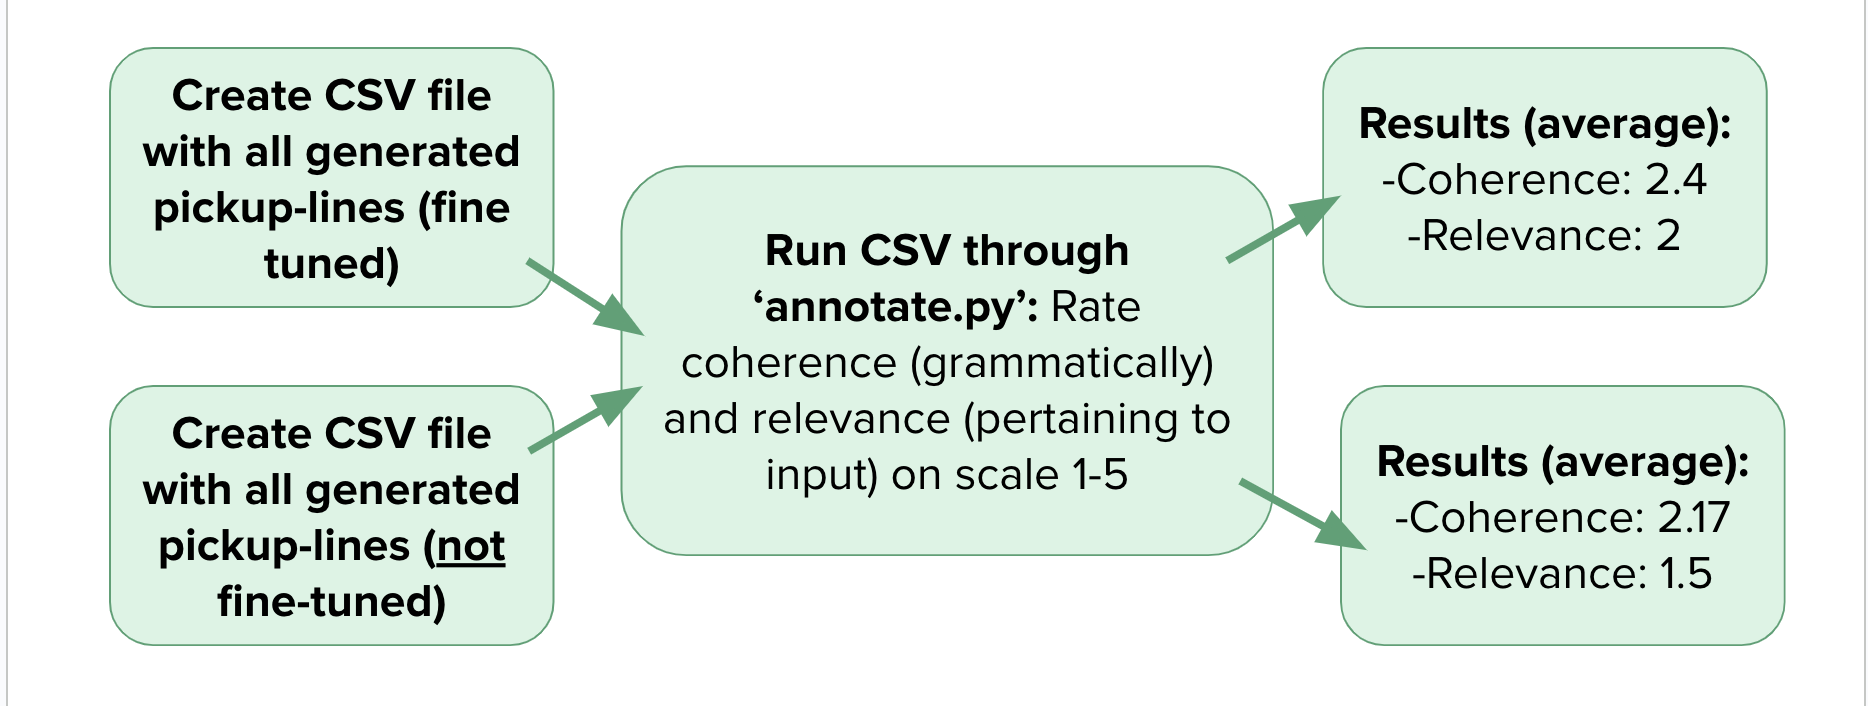
\includegraphics[width=0.75\textwidth]{pictures/evaluate.png}
\caption{Summary of evaluation methods.}
\end{figure}

In order to create a portion of our project that was interactive for users, we created a Flask app to generate pickup lines using our 'fine\_tuned.py' and 'generation.py' files. First, we created the following 3 files:
\begin{itemize}
    \item \textit{app.py}: The main code for creating the flask app.
    \item \textit{index.html}: Populate the app with a place for user input and the 'generate' button to call our functions.
    \item \textit{results.html}: Populate the page after the user inputs something with the 2 generated pickup lines.
\end{itemize}

Once we run the 'app.py' file, the flask app can run in an external port by pasting the 'http' string in a web browser. Once reaching the app, the user is prompted to enter the beginning of a pickup line (a question or half of a sentence) and our app will return an answer or the other half of the sentence. Note, we manually entered the path for our fine tuned model in this file, so if you would like to run the app on your own computer you should be sure to change this to the appropriate path. In order to directly take in user input, we had to modify our 'generation.py' file to include a new function 'generate\_pickup\_lines' that specifically tokenizes the 'start\_text' which is what we labeled the user input to be. We also decode the generated pickup lines within this function instead of waiting until we print the output (the following function in our original 'generation.py' file). This allows us to only have to import the 'generate\_pickup\_lines' function and not necessarily the entire 'generation.py' file, simplifying the generation process. Once the generation occurs, the screen of the port running the flask app changes to display the outputs. Below we have included screenshots of both screens of our app for the user input 'my love for you is like a loop':

\begin{figure}[H]
\centering
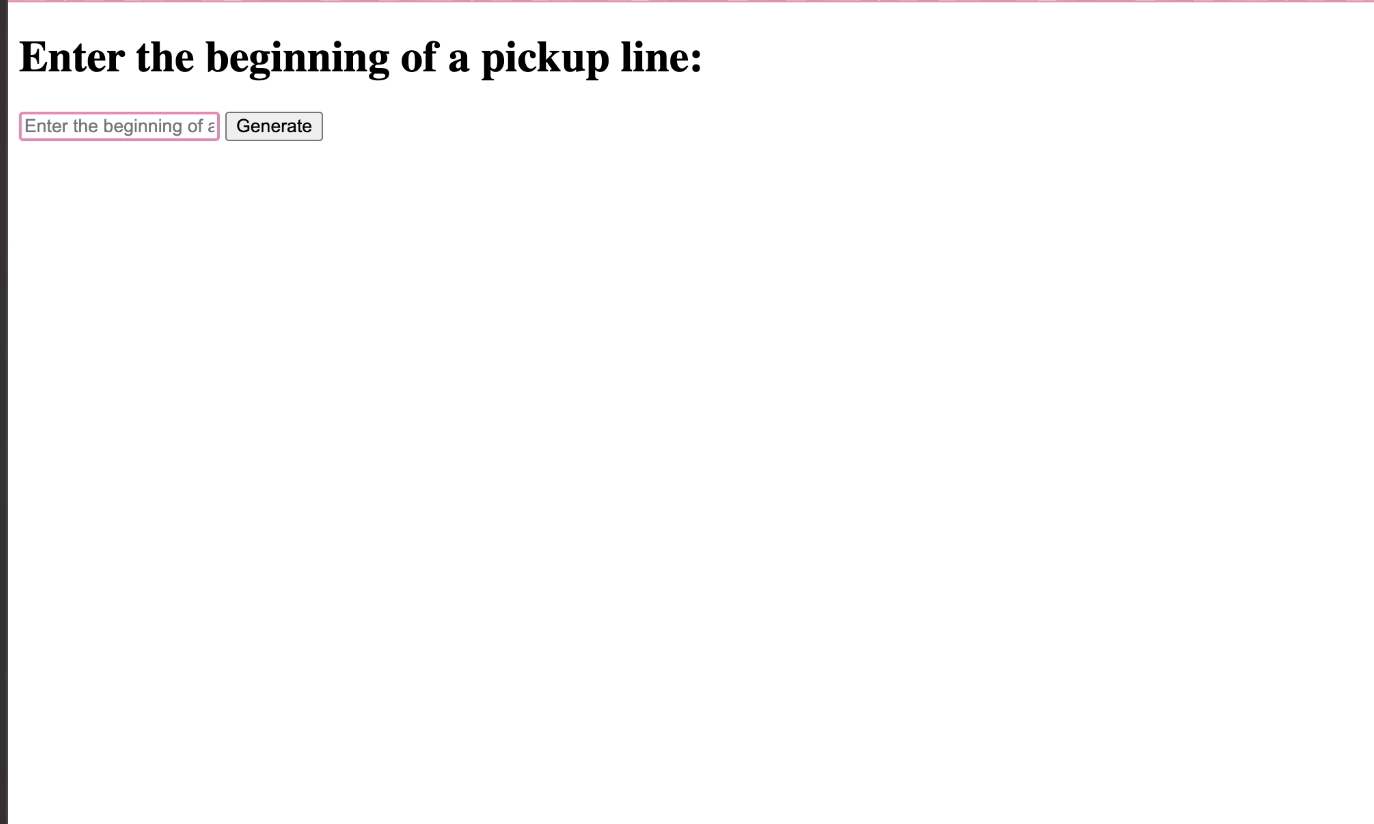
\includegraphics[width=0.8\textwidth]{pictures/flask pg1.png}
\caption{User Input Screen}
\end{figure}



\begin{figure}[H]
\centering
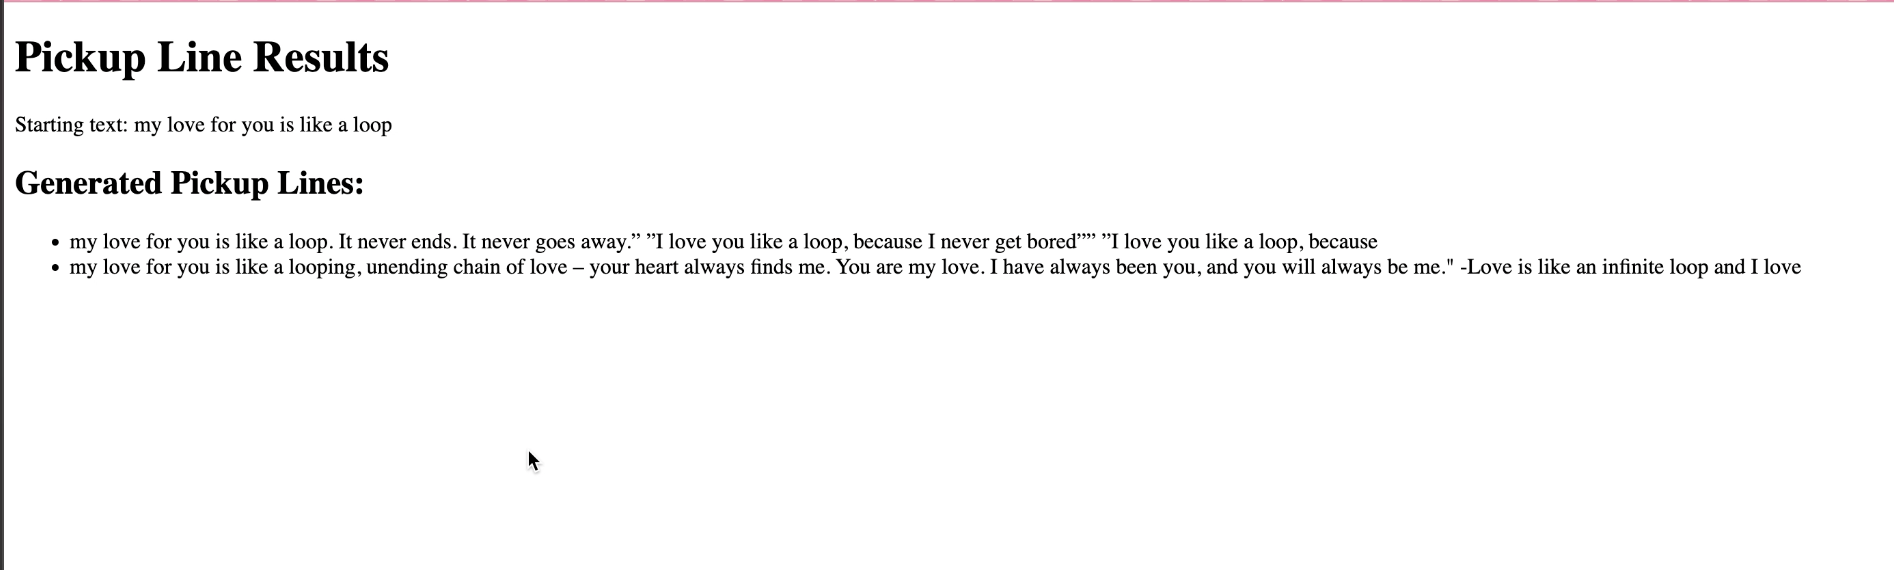
\includegraphics[width=1\textwidth]{pictures/flask pg2.png}
\caption{Output Screen}
\end{figure}


Taking a look at some of our generated pickup lines with our fine-tuned model, we can observe the input and output as seen below, where all 5 of these examples were rated with a 5 for coherence and for relevance.

\begin{table}[H]
    \centering
\begin{tabularx}{0.8\textwidth} { 
  | >{\raggedright\arraybackslash}X 
  | >{\raggedright\arraybackslash}X  | }
  \hline
 \textbf{Input}  & \textbf{Output}  \\
 \hline
 Are you a graph? & Are you a graph? Because you’ve got my heart all connected. It's a pattern of mathematical equations. Every time I see it, my heart goes a little faster.I don't know if it’s \\
 \hline
 Your must be a compiler because  & Your must be a compiler because you make my code look like an assembly! $<3 <3 <3 <3 <3 <3 <3 <3 <3 <3 <3 <3 <3 <3 <3 <3 <3$   \\
 \hline
 Are you GitHub?  & Because I'm looking up your status! Because you're my favorite project repository! Because you're always working on the same thing, so you end up getting the most work done! Because you're like a computer, you can always  \\
  \hline
 My love for you is like a fractal because  & My love for you is like a fractal because you have infinite growth, and I can never stop growing. You have my entire heart, and your beauty is a miracle. I cannot express my love for you without growing your love. Because you are \\
  \hline
 Are you a Wi-Fi signal?  & Are you a Wi-Fi signal? Because you’re getting more and more connected with me. I’m seeing you in my heart.” ‪I’m feeling connected with you.”  \\
  \hline
\end{tabularx}
    \caption{Fine-Tuned Model Generation Examples - High Rating}
    \label{tab:my_label}
\end{table}

Interestingly, we can examine some examples of the non-fine tuned model to compare and see how effective our fine-tune training was! Specifically looking at the first and third examples, we have direct comparisons to the fine-tuned model. We seem to have successfully trained our model to generate pickup-style lines!!

\begin{table}[H]
    \centering
\begin{tabularx}{0.8\textwidth} { 
  | >{\raggedright\arraybackslash}X 
  | >{\raggedright\arraybackslash}X  | }
  \hline
 \textbf{Input}  & \textbf{Output}  \\
 \hline
 Are you a graph? & Are you a graph? Yes. What kind of graph? A graph is a collection of data that is organized into a tree structure. How many trees does it have? It can be as many as \\
 \hline
 Are you a CPU?  & Are you a CPU? If you're a GPU, you can use the GTX 680 and GTX 770 graphics cards and do some heavy computation on any video game or game engine, but you'll need to know how to do it on AMD.   \\
 \hline
 Are you GitHub?  & Are you GitHub? Because, why not? If you're an expert in Git, you might want to read this: GitHub: the best project management tool for the modern web. It's a useful book, so I'll leave  \\
  \hline
\end{tabularx}
    \caption{Non Fine-Tuned Model Generation Examples}
    \label{tab:my_label}
\end{table}



\section{Conclusion}
In the hopes of helping STEM majors develop their social skills, we have created the ultimate pickup line generator tool: the \textit{PickupMaster 9000}. We fine-tuned the pretrained LLM GPT-2 using CS and math pickup lines gathered from various internet sources, and were able to subsequently generate new pickup lines in the expected format. In the process of training our model, we learned what hyperparameters worked best with our Trainer, as well as parameters and decoding strategy with our generation. In general, we have gained a deeper understanding of word generation tasks and fine-tuning PLM's. In the future, we would like to further develop our human annotation by incorporating a custom loss function to use these scores to further fine-tune our model. Our evaluation metrics would also be less biased with more people scoring the generated lines. We would also like to explore more combinations of all the hyperparameters with more time, possibly by using grid search. Additionally, we would like to see if our model improves with even more training data, and it would be interesting to make separate models for different categories. Overall, we demonstrated success in generating pickup lines much better than a pretrained language model alone without fine tuning, and we can't wait for our friends to use it!


\bibliographystyle{plain}
\bibliography{references}

\section{data websites}
\href{https://wittypro.net/pick-up-lines/computer-programming-pick-up-lines-and-rizz/}{1. Wittypro}

\href{https://www.reddit.com/r/ProgrammerHumor/comments/oz77xb/programmer_pickup_lines_ive_collected_these_past/ }{2. Reddit}

\href{https://punsteria.com/computer-science-puns/  }{3. Punsteria}

\href{https://attractmorematches.com/computer-science-pick-up-lines/}{4. Attract More Matches}

\href{https://pickupline.net/academic-pick-lines/computer-programming-pick-up-lines/ }{5. Pickupline}

\href{https://www.rd.com/article/math-pickup-lines/ }{6. RD}

\href{https://www.reddit.com/r/math/comments/gy66d4/i_need_every_one_of_your_corniest_mathy_pick_up/ }{7. Reddit}

\href{https://thoughtcatalog.com/january-nelson/2021/05/math-pick-up-lines/ }{8. Thought Catalog}

\href{https://www.mashupmath.com/blog/math-pickup-lines }{9. Mashup Math}

\href{https://www.boredpanda.com/math-pick-up-lines/ }{10. Bored Panda}

\href{https://ponly.com/math-pickup-lines/ }{11. Ponly}

\href{https://www.weareteachers.com/math-jokes/}{12. We Are Teachers}

\end{document}
